\documentclass[a4paper]{article}
\usepackage{tikz}

\begin{document}
We are working on \tikz \draw[step=2pt] (0,0) grid (10pt,10pt);

\tikzset{help lines/.style={very thin,color=blue!50}}

\tikzset{Karl’s grid/.style={help lines,color=blue!50}}

\begin{tikzpicture}
	[Karl’s grid/.style = {help lines,color=#1!50}, Karl’s grid/.default=blue]
	\draw[Karl’s grid] (0,0) grid (1.5,2);
	\draw[Karl’s grid=red] (2,0) grid (3.5,2);
\end{tikzpicture}

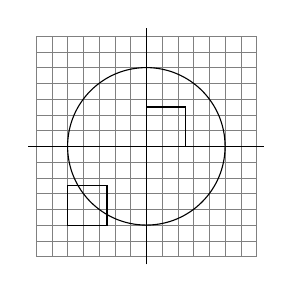
\begin{tikzpicture}
%  help lines/.style={color=blue,very thin}
	\draw [step=0.2cm, help lines] (-1.4,-1.4) grid (1.4,1.4);
	\draw (-1.5,0) -- (1.5,0);
	\draw (0,-1.5) -- (0,1.5);
	\draw (0,0) circle (1cm);
	\draw (0,0) rectangle (0.5,0.5);
	\draw (-0.5,-0.5) rectangle (-1,-1);
\end{tikzpicture}

\begin{tikzpicture}
	\draw[Karl’s grid] (0,0) grid (3,3);
\end{tikzpicture}

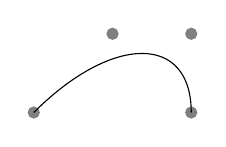
\begin{tikzpicture}
	\filldraw [gray] (0,0) circle (2pt)
	(1,1) circle (2pt)
	(2,1) circle (2pt)
	(2,0) circle (2pt);
	\draw (0,0) .. controls (1,1) and (2,1) .. (2,0);
\end{tikzpicture}

\begin{tikzpicture}
	\draw [fill=gray, gray] (0,0) circle (2pt)
	(1,1) circle (2pt)
	(2,1) circle (2pt)
	(2,0) circle (2pt);
\end{tikzpicture}

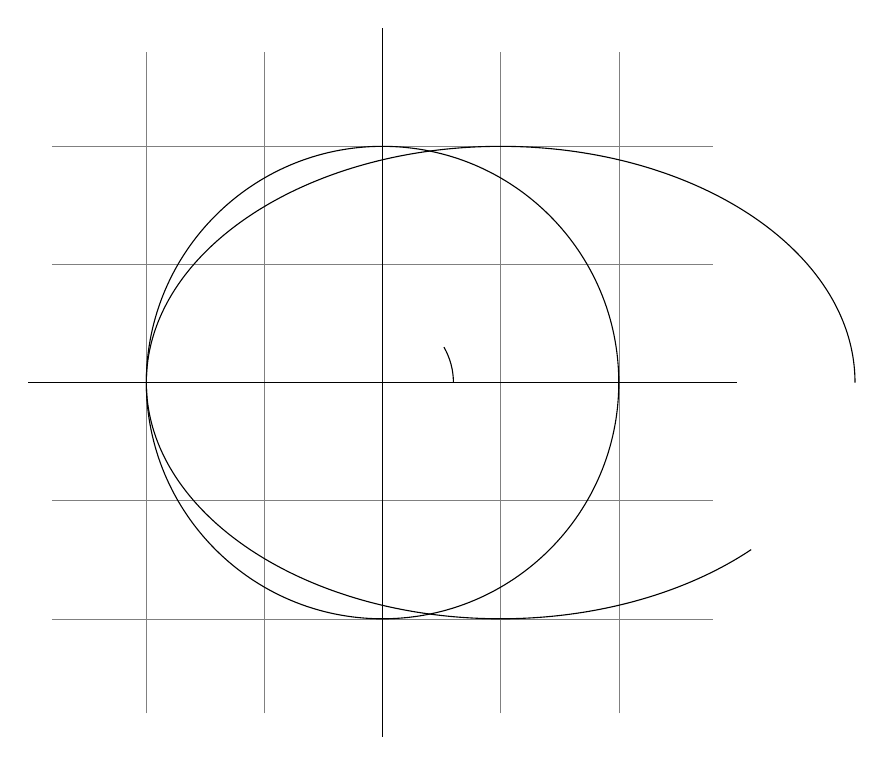
\begin{tikzpicture}[scale=3]
  \draw[step=0.5cm, help lines] (-1.4,-1.4) grid (1.4,1.4);
  \draw (-1.5,0) -- (1.5,0);
  \draw (0,-1.5) -- (0,1.5);
  \draw (0,0) circle (1cm);
  \draw (3mm,0mm) arc (0:30:3mm);
  \draw (2,0) arc (0:315:1.5cm and 1cm);
\end{tikzpicture}

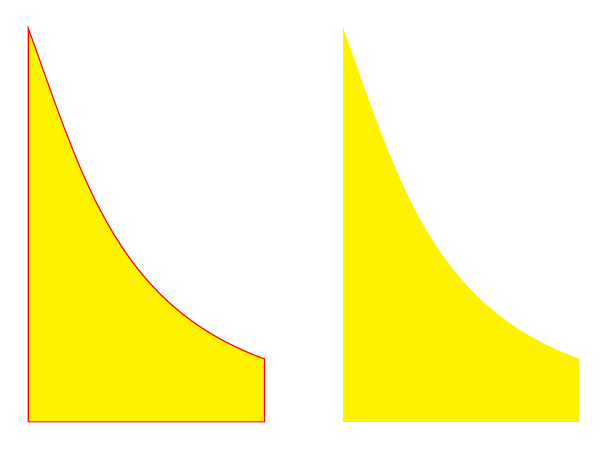
\begin{tikzpicture}
  \draw[red, fill=yellow](0,0) -- (0,5) to [out=290,in=160] (3,0.8) -- (3,0) -- (0,0);
  \path[fill=yellow](4,0) -- (4,5) to [out=290,in=160] (7,0.8) -- (7,0) -- (4,0);
\end{tikzpicture}

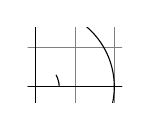
\begin{tikzpicture}
  \clip (-0.1,-0.2) rectangle (1.1,0.75);
  \draw[step=0.5, help lines] (-1.4,-1.4) grid (1.4,1.4);
  \draw (-1.5,0) -- (1.5,0);
  \draw (0,-1.5) -- (0,1.5);
  \draw (0,0) circle (1cm);
  \draw (3mm,0mm) arc (0:30:3mm);
\end{tikzpicture}

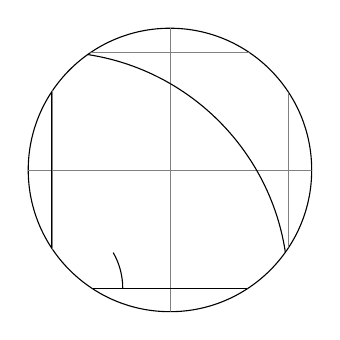
\begin{tikzpicture}[scale=3]
	%\clip[draw] (0.5,0.5) circle (0.6cm);
	\draw[clip] (0.5,0.5) circle (0.6cm);
	\draw[step=.5cm,gray,very thin] (-1.4,-1.4) grid (1.4,1.4);
	\draw (-1.5,0) -- (1.5,0);
	\draw (0,-1.5) -- (0,1.5);
	\draw (0,0) circle (1cm);
	\draw (3mm,0mm) arc (0:30:3mm);
\end{tikzpicture}

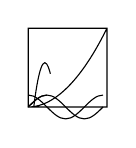
\begin{tikzpicture}
	\draw (0,0) rectangle (1,1) (0,0) parabola (1,1);
	\draw[x=1pt,y=1pt] (2,0) parabola bend (6,16) (8,12);
%	\draw (2,0) parabola bend (6,16) (8,12);
	\draw[x=1ex,y=1ex] (0,0) sin (1.57,1);
	\draw[x=1.57ex,y=1ex] (0,0) sin (1,1) cos (2,0) sin (3,-1) cos (4,0)
												(0,1) cos (1,0) sin (2,-1) cos (3,0) sin (4,1);
\end{tikzpicture}

\tikzset{help lines/.style={very thin,color=black}}
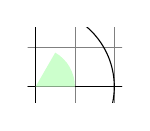
\begin{tikzpicture}
  \clip (-0.1,-0.2) rectangle (1.1,0.75);
  \draw[step=0.5cm, help lines] (-1.4,-1.4) grid (1.4,1.4);
  \draw (-1.5,0) -- (1.5,0);
  \draw (0,-1.5) -- (0,1.5);
  \draw (0,0) circle (1cm);
  \fill[green!20!white] (0,0) -- (0.5cm,0cm) arc (0:60:0.5cm) -- (0,0);
\end{tikzpicture}

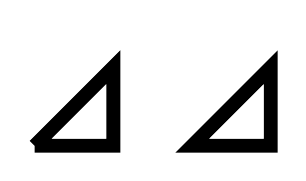
\begin{tikzpicture}[line width=5pt]
	\draw (0,0) -- (1,0) -- (1,1) -- (0,0);
	\draw (2,0) -- (3,0) -- (3,1) -- cycle;
	\useasboundingbox (0,1.5); % make bounding box higher
\end{tikzpicture}

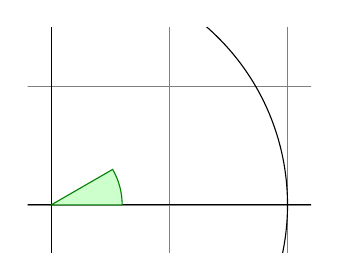
\begin{tikzpicture}[scale=3]
	\clip (-0.1,-0.2) rectangle (1.1,0.75);
	\draw[step=.5cm,gray,very thin] (-1.4,-1.4) grid (1.4,1.4);
	\draw (-1.5,0) -- (1.5,0);
	\draw (0,-1.5) -- (0,1.5);
	\draw (0,0) circle (1cm);
	\filldraw[fill=green!20!white, draw=green!50!black] (0,0) -- (3mm,0mm) arc (0:30:3mm) -- cycle;
\end{tikzpicture}

\end{document}
